\subsection{Client-Server}
Durch ihre dynamische Struktur kann die Pipeline auf einer weiteren
Abstraktionsschicht durch das \first{Client-Server}-Pattern dargestellt werden:
Ein statischer Server kommuniziert über eine definierte Schnittstelle mit
dynamischen Clients.
Clients können kommen und gehen und sind nicht auf eine konkrete
Implementierung festgelegt. 

Die \first{Pipes} des \name{pipes and filters} Pattern werden somit zu einem
zentralen \first{Server} zusammengefasst und bilden das statische
Ausführungsgerüst.
\first{Clients} werden durch die \first{Steps} repräsentiert. \seec{chp:pipes
and filters} Es können beliebig viele Clients am Server anmeldet werden, wodurch
die eigentliche Pipeline aufgebaut wird.

\begin{figure}[htbp]
	\begin{center}
		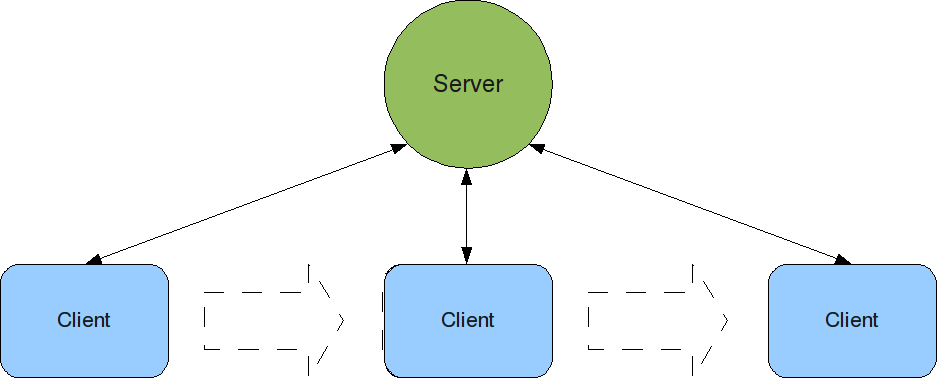
\includegraphics[scale=0.6]{pics/serverClient2.png}
	\caption[Client Server]{
	\textbf{Abstraktion durch das Client-Server-Pattern.}
	Einzelne \name{Steps} können sich
	dynamisch an einem \name{Server} an- und abmelden. Der Server organisiert die
	angemeldeten Clients nach deren Anmeldung zu der eigentlichen Pipeline.}
	\end{center}
	\label{fig:clientServer2}
\end{figure}

\paragraph{Server}
Die Anforderungen an den Server gliedern sich in zwei Teilbereiche:
\begin{description}
\item[Organisation und Synchronisation der Client Ausführung]
Die Ausfürhrung der angemeldeten Steps kann sequenziell oder
parallel erfolgen, je nachdem, welche \name{preconditions} für den jeweiligen
Step erforderlich sind und ob die zur Ausführung benötigten Daten eventuell
erst durch einen anderen Step bereitgestellt werden müssen.
Vor der eigentlichen Ausführung wird der Server somit zum einen die
\name{preconditions} prüfen, zum anderen, ob der Step überhaupt zur Ausführung
gebracht werden muss, oder ob die zu erwartenden Ergebnisse bereits in selber
oder in anderer Form vorhanden sind.
\item[Datenverwaltung] Die Ergebnisse der einzelnen Steps werden zentral durch
den Server verwaltet.
Zum einen synchronisiert der Server die Zugriffe auf die Daten, zum anderen
werden diese persistiert, um bei einer gewollten oder ungewollten Unterbrechung
der Pipeline Datenverlust zu verhindern.
\end{description}

\paragraph{Client}
Auf der Clientseite stehen die einzelnen Steps, die eine gemeinsame
Schnittstelle zur Kommunikation mit dem Server implementieren über welche der
Server \name{preconditions} überprüfen, \name{solutions}
\seec{chp:softwarearchitektur} entgegennehmen und die eigentliche Ausführung
anstossen kann.

%%
%\begin{figure}[htbp]
%	\begin{center}
%		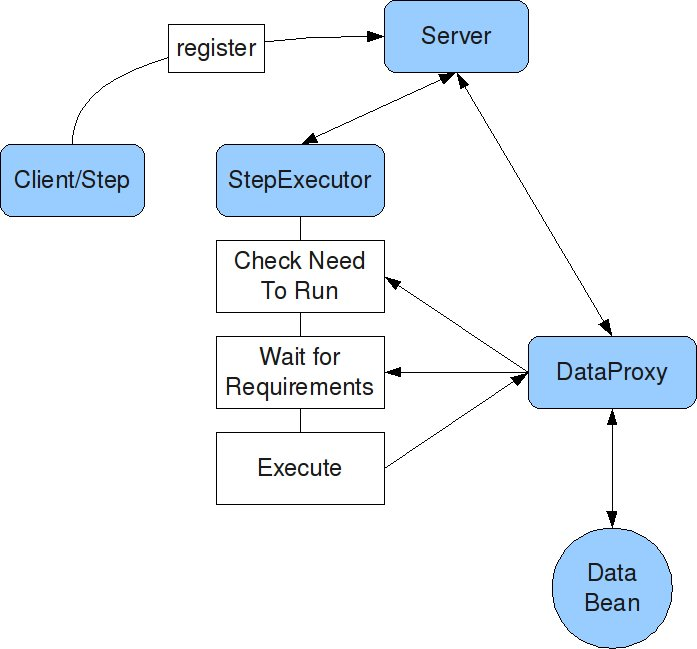
\includegraphics[scale=0.6]{pics/programOrganisationOverview3ScaledWithAlpha.jpg}
%	\caption[Design 1]{
%	\textbf{Design 1.}
%	something. \todo{Teilung von Server hier noch nicht erwähnt. Evtl. Teil der
%	Umstzung}}
%	\end{center}
%	\label{fig:programOrganisationOverview3ScaledWithAlpha}
%\end{figure}